\documentclass[aps,prb,twocolumn,superscriptaddress,floatfix,longbibliography,10pt]{revtex4-2}

\usepackage[utf8]{inputenc}
\usepackage[spanish]{babel}
\usepackage{graphicx}
\usepackage{amsmath}
\usepackage{subcaption}
\usepackage{wrapfig} 
\usepackage[export]{adjustbox}

\usepackage{amsmath,amssymb} % math symbols
\usepackage{bm} % bold math font
\usepackage{graphicx} % for figures
\usepackage{comment} % allows block comments
\usepackage{textcomp} % This package is just to give the text quote '
%\usepackage{ulem} % allows strikeout text, e.g. \sout{text}

\usepackage[spanish]{babel}
% By dafault, spanish changes to a comma as decimal separator; to change to a dot, you can use \decimalpoint:
\decimalpoint

\usepackage{enumitem}
\setlist{noitemsep,leftmargin=*,topsep=0pt,parsep=0pt}

\usepackage{xcolor} % \textcolor{red}{text} will be red for notes
\definecolor{lightgray}{gray}{0.6}
\definecolor{medgray}{gray}{0.4}

%Para las tablas
\usepackage{multirow}

\usepackage{hyperref}
\hypersetup{
colorlinks=true,
urlcolor= blue,
citecolor=blue,
linkcolor= blue,
bookmarks=true,
bookmarksopen=false,
}

% Code to add paragraph numbers and titles
\newif\ifptitle
\newif\ifpnumber
\newcounter{para}
\newcommand\ptitle[1]{\par\refstepcounter{para}
{\ifpnumber{\noindent\textcolor{lightgray}{\textbf{\thepara}}\indent}\fi}
{\ifptitle{\textbf{[{#1}]}}\fi}}
% \ptitletrue  % comment this line to hide paragraph titles
% \pnumbertrue  % comment this line to hide paragraph numbers

% minimum font size for figures
\newcommand{\minfont}{6}

% Uncomment this line if you prefer your vectors to appear as bold letters.
% By default they will appear with arrows over them.
% \renewcommand{\vec}[1]{\bm{#1}}

%Cambiar Cuadros por Tablas y lista de...
%\renewcommand{\listtablename}{Índice de tablas}
\renewcommand{\tablename}{Tabla}
\renewcommand{\date}{Fecha}

%Para importar imágenes desde una carpeta:
\graphicspath{ {C:/Users/lupam/OneDrive/Escritorio/GitHub/Metodos_Num_Fluidos_I/Guias/Guia_3/ejercicio_6/Programa/graficos} {C:/Users/lupam/OneDrive/Escritorio/GitHub/Metodos_Num_Fluidos_I/Guias/Guia_3/ejercicio_6/Informe/Figures}}


\usepackage[bottom]{footmisc} %para que las notas al pie aparezcan en la misma página

\begin{comment}

%Comandos de interés:

* Para ordenar el documento:
\section{Introducción}
\section{\label{sec:Formatting}Formatting} %label para luego hacer referencia a esa sección

\ptitle{Start writing while you experiment} %pone nombre y título al documento dependiendo de si en el header están los comandos \ptitletrue y \pnumbertrue

* Ecuaciones:
\begin{equation}
a^2+b^2=c^2 \,.
\label{eqn:Pythagoras}
\end{equation}

* Conjunto de ecuaciones:
\begin{eqnarray}
\label{eqn:diagonal}
\nonumber d & = & \sqrt{a^2 + b^2 + c^2} \\
& = & \sqrt{3^2+4^2+12^2} = 13
\end{eqnarray}

* Para hacer items / enumerar:
\begin{enumerate}
  \item
\end{enumerate}

\begin{itemize}
  \item
\end{itemize}

* Figuras:
\begin{figure}[h]
    \includegraphics[clip=true,width=\columnwidth]{pixel-compare}
    \caption{}
     \label{fig:pixels}
\end{figure}

* Conjunto de figuras:
(no recuerdo)


* Para hacer referencias a fórmulas, tablas, secciones, ... dentro del documento:
\ref{tab:spacing}

* Para citar
Elementos de .bib
\cite{WhitesidesAdvMat2004}
url
\url{http://www.mendeley.com/}\\

* Agradecimientos:
\begin{acknowledgments}
We acknowledge advice from Jessie Zhang and Harry Pirie to produce Fig.\ \ref{fig:pixels}.
\end{acknowledgments}

* Apéndice:
\appendix
\section{\label{app:Mendeley}Mendeley}

* Bibliografía:
\bibliography{Hoffman-example-paper}

\end{comment}



\begin{document}

% Allows to rewrite the same title in the supplement
\newcommand{\mytitle}{Laboratorio 3 - \textcolor{red}{??}}

\title{\mytitle}

\author{Pablo Chehade \\
    \small \textit{pablo.chehade@ib.edu.ar} \\
    \small \textit{Métodos Numéricos en Fluidos I, Instituto Balseiro, CNEA-UNCuyo, Bariloche, Argentina, 2022} \\}


\begin{abstract}

Se resolvió numéricamente la ecuación de onda escalar, homogénea y unidimensional con velocidad dependiente de la posición. En concreto, se empleó el método Runge-Kutta 4 para la evolución temporal y diferencias finitas de orden 2 para la espacial. Se analizó la evolución temporal de una condición inicial para distintas funciones de velocidad. Se estudió la estabilidad de la solución y se determinó la relación entre la velocidad y las discretizaciones espaciales y temporales, de modo de asegurar estabilidad. Esto se realizó mediante el análisis del número de onda modificado y se verificó numéricamente para distintas funciones de velocidad.

\end{abstract}

\maketitle

\section{Introducción}

En ciencias físicas es usual modelar sistemas mediante ecuaciones diferenciales en derivadas parciales. Algunas ecuaciones cuentan con dependencias tanto espaciales como temporales, tratándose representativamente de un problema de valores de contorno para la dependencia espacial y uno de valores iniciales para la temporal. Sin embargo, no toda ecuación cuenta con solución analítica y es necesario recurrir a aproximaciones. De este modo, es necesario proponer un método numérico para cada dependencia. Esto implica que a las ventajas y desventajas propias de cada método se le suman nuevas propias de la combinación de métodos, lo cual debe ser estudiado en detalle para cada problema en particular.

En este trabajo se resolvió numéricamente una ecuación diferencial particular y se estudió las características de la solución en base a los métodos empleados. En particular, se resolvió la ecuación de onda escalar, homogénea y unidimensional
\begin{equation}
  \frac{\partial^2 u}{\partial t^2} = c^2(x)\frac{\partial^2 u}{\partial x^2} \,, t \geq 0, \,  0 < x < 4,
  \label{eq:ecuacion_ondas}
\end{equation}
con condiciones iniciales
\begin{equation}
  \left\{\begin{matrix}
    u(x,0) = u_0(x) = e^{-200 (x-0.25)^2} \\
    u_t(x,0) = 0
   \end{matrix}\right.
  \label{eq:condiciones_iniciales}
\end{equation}
y condiciones de contorno
\begin{equation}
  \left \{\begin{matrix}
    \left . \frac{\partial u}{\partial t} \right |_{x=0} = c(0) \left . \frac{\partial u}{\partial x} \right |_{x=0} ,\\
    \left . \frac{\partial u}{\partial t} \right |_{x=4} = - c(4) \left . \frac{\partial u}{\partial x} \right |_{x=4},
   \end{matrix}\right .
  \label{eq:condiciones_contorno}
\end{equation}
para una variedad de velocidades del sonido $c(x)$ en el medio. Una particularidad de la ecuación es la ausencia de término difusivo, por lo que una onda en un medio homogéneo se transmite sin modificar su amplitud. \textcolor{red}{Esto es así?}. 

% La ecuación de onda es de gran importancia en ciencias físicas debido a que describe la propagación de una gran diversidad de ondas. Con ella es posible modelar ondas sonoras, ondas de luz, ondas en medios fluidos, entre otras. Aunque no solo permite simular la propagación en un medio homogéneo, sino también la reflexión y transmisión al cambiar de medio, lo cual suele representarse como un cambio en la velocidad de propagación.

% Una particularidad de la ecuación es la ausencia de término difusivo, por lo que una onda en un medio homogéneo se transmite sin modificar su amplitud. \textcolor{red}{Esto es así?}. Por otro lado, este estudio debió hacerse numéricamente debido a que no siempre es posible obtener una solución analítica para cualquier dependencia espacial de la velocidad.

\section{Métodos Numéricos}

La ecuación de onda \ref{eq:ecuacion_ondas} de segundo orden en el tiempo se puede transformar en el siguiente sistema de ecuaciones de primer orden en el tiempo mediante el cambio de variables $u_a = u$, $u_b = \partial u /\partial t$
\[
  \left \{ \begin{matrix}
     \frac{\partial u_a}{\partial t} = u_b   \\
     \frac{\partial u_b}{\partial t} = c^2(x) \frac{\partial^2 u_a}{\partial x^2}
  \end{matrix} \right .
  \]
junto a las condiciones iniciales
\[ \left \{ \begin{matrix}
     u_a(x,0) = u_0(x) \\
     u_b(x,0) = 0
  \end{matrix} \right .
\]  
y a las condiciones de borde
\[
  \left \{ \begin{matrix}
     \left . \frac{\partial u_a}{\partial t} \right |_{x=0} = c(0) \left . \frac{\partial u_a}{\partial x} \right |_{x=0} ,\\
     \left . \frac{\partial u_a}{\partial t} \right |_{x=4} = - c(4) \left . \frac{\partial u_a}{\partial x} \right |_{x=4},
  \end{matrix} \right .
\]

Para resolver numéricamente el sistema, es necesario discretizar el dominio y proponer métodos numéricos para la parte espacial y temporal, buscando asegurando la estabilidad de la solución.

En cuanto a la discretización del dominio, la variable espacial se discretizó en puntos equiespaciados $x_j = \Delta x * j$ donde $j = 1,\dots,M$ y $\Delta x = 1/(M+1)$. Por otro lado, la variable temporal también se discretizó en puntos equiespaciados $t_n = \Delta t * n$ con $n = 0,1,\dots,N$ y $\Delta t = 1/N$.

En cuanto al método numérico para la variable espacial, se empleó diferencias centradas de orden dos para los nodos internos
\[\frac{\partial^2 u_j}{\partial x^2} = \frac{u_{j+1} - 2 u_j + u_{j-1}}{\Delta x^2} + O(\Delta x^2),  \]
diferencias finitas adelantada orden 2 para el nodo del borde izquierdo ($j = 0$) \textcolor{red}{Referencia al Moin}
\[\left . \frac{\partial u}{\partial x} \right |_0 = \frac{-3 u_0 + 4 u_{1} - u_{2}}{2 \Delta x} + O(\Delta x^2) \]
y diferencias finitas atrasada de orden 2 para el nodo del borde derecho ($j = N + 1$) \textcolor{red}{referencia a wikipedia}
\[\left . \frac{\partial u}{\partial x} \right |_{N+1} = \frac{3 u_{N+1} - 4 u_N + u_{N-1}}{2 \Delta x} + O(\Delta x^2) \]
En base a estas aproximaciones, el sistema de ecuaciones junto a las condiciones de borde se convierten en el sistema semidiscretizado \textcolor{red}{Corroborar la expresión}
\begin{equation}
  \left \{ \begin{matrix}
   \frac{\partial u_{a j}}{\partial t} = u_{b j} \\
   \frac{\partial u_{b j}}{\partial t} = \frac{c_j^2}{\Delta x^2} (u_{a j+1} - 2 u_{a j} + u_{a j-1}) \\
   \frac{\partial u_{a 0}}{\partial t} = \frac{c(0)}{2 \Delta x} (-3 u_{a 0} + 4 u_{a 1} - u_{a 2}) \\
   \frac{\partial u_{a N+1}}{\partial t} = \frac{c(4)}{2 \Delta x} (-3u_{a N+1} + 4 u_{a N} - u_{a N-1}) 
  \end{matrix} \right .
  \label{eq:sistema_semi_discretizado}
\end{equation}


donde $c_j = c(x_j)$. De este modo, para nodos internos se tienen dos ecuaciones diferenciales con dos incógnitas ($u_a$ y $u_b$). Mientras que para los nodos de borde se tiene una ecuación diferencial con una incógnita ($u_a$). Este sistema se puede escribir de la forma
\[\frac{d \vec{z}}{dt} = \gamma \vec{z} = \vec{f}(\vec{z},t)\]
definiendo el vector $\vec{z}$ tal que $\vec{z}^T = (u_{a 0}, u_{a 1}, \dots, u_{a N}, u_{a N+1}, u_{b 1}, u_{b 2}, \dots, u_{b N+1})$ y la matriz
\[\gamma = \begin{pmatrix}
  A & B \\
  C & D \\
  \end{pmatrix}\]
tal que
\[A = \frac{1}{2 \Delta x} \begin{pmatrix}
  -3c(0) & 4c(0) & -c(0) & 0 & \cdots & 0 \\ \\
  & & 0_{Nx(N+2)} & &\\ \\
  0 & \cdots & 0 & -c(4) & 4c(4) & -3c(4) \\
  \end{pmatrix} \]
\[B = \begin{pmatrix}
  0 & \cdots & 0 \\ \\
  & I_{NxN} & \\ \\
  0 & \cdots & 0 \\
  \end{pmatrix}
   \]
\[ C = \frac{1}{\Delta x^2} \begin{pmatrix}
  c_1^2 & -2 c_1^2 & c_1^2 & 0 & \cdots & 0 \\
  0 & c_2^2 & - 2 c_2^2 & c_2^2 & \cdots & 0 \\
  \vdots & \vdots & \ddots & \ddots & \ddots & \vdots \\
  0 & \cdots & 0 & c_N^2 & - 2 c_N^2 & c_N^2
  \end{pmatrix} \]
\[ D =  0_{NxN}\]

En cuanto a la variable temporal se empleó el método Runge-Kutta de orden 4
\begin{equation}
  \nonumber \vec{z}_{n+1} = \vec{z}_n + \frac{1}{6} \vec{k}_1 + \frac{1}{3} (\vec{k}_2 + \vec{k}_3) + \frac{1}{6} \vec{k}_4 + O_{local}(h^5)
  \label{eq:Runge_Kutta_4}
\end{equation}
donde
\[
  \left\{\begin{matrix}
    \vec{k}_1 = h \vec{f}(\vec{z}_n, t_n), \\ 
    \vec{k}_2 = h \vec{f} \left( \vec{z}_n + \frac{1}{2} \vec{k}_1 , t_n + \frac{h}{2}\right), \\
    \vec{k}_3 = h \vec{f} \left ( \vec{z}_n + \frac{1}{2} \vec{k}_2 , t_n + \frac{h}{2}  \right ), \\
    \vec{k}_4 = h \vec{f}(\vec{z}_n + \vec{k}_3, t_n + h)
  \end{matrix}\right.
\]

Como se mencionó anteriormente, debido a la combinación de métodos realizados pueden aparecer nuevos problemas de convergencia. En particular, puede cambiar la estabilidad de la solución dependiendo de los valores de $\Delta x$ y $\Delta t$ elegidos. Para esto es útil realiar el análisis con número de onda modificado, el cual se basa en proponer soluciones del tipo
\[a \]
en el sistema de ecuaciones semi-discretizado \ref{eq:sistema_semi_discretizado} ignorando las condiciones de contorno. Realizando el reemplazo y desarrollando las ecuaciones se obtiene un sistema de ecuaciones
\[ \]
donde $\lambda$ es la matriz
\[solo la matriz\]
con autovalores $\chi$

En este momento es necesario especificar el método numérico te

Resumen de lo que se hará


\section{Resultados y discusión}

\textcolor{red}{Inestabilidad por el paso de tiempo porque las oscilaciones espúreas son acotadas ¿Por qué no obtengo oscilaciones espúreas? Hay oscilaciones espúreas en el caso de pe>2 si hubiera difusión. PERO NO HAY DIFUSIÓN. Aparecerían si la grilla es grande y la solución es empinada. Usar un $N = 100$.}

\begin{figure}[h]
  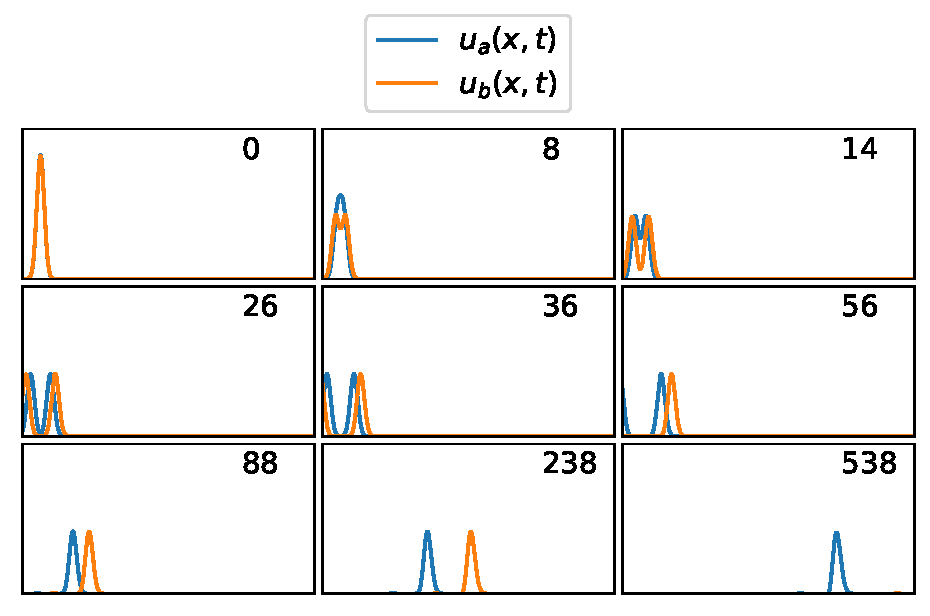
\includegraphics[clip=true,width=\columnwidth]{solucion_a_y_c.pdf}
  \caption{Distintos instantes de la evolución de la solución para distintas funciones de velocidad. $u_a(x,t)$ corresponde a la velocidad constante $c_a(x) = 1$, mientras que $u_b(x,t)$ corresponde a la velocidad constante $c_b(x) = 1.5$. El \textcolor{red}{numerito indica el índice n. Agregar Deltax y deltat}}. 
   \label{fig:solucion_a_y_c}
\end{figure}

\begin{figure}[h]
  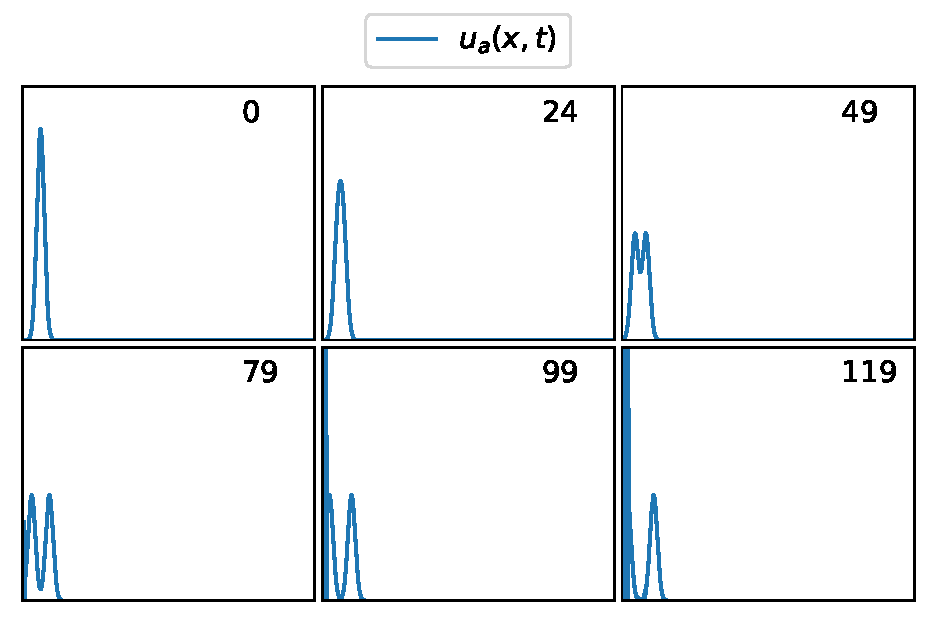
\includegraphics[clip=true,width=\columnwidth]{solucion_a_divergente.pdf}
  \caption{}
   \label{fig:solucion_a_divergente}
\end{figure}

\begin{figure}[h]
  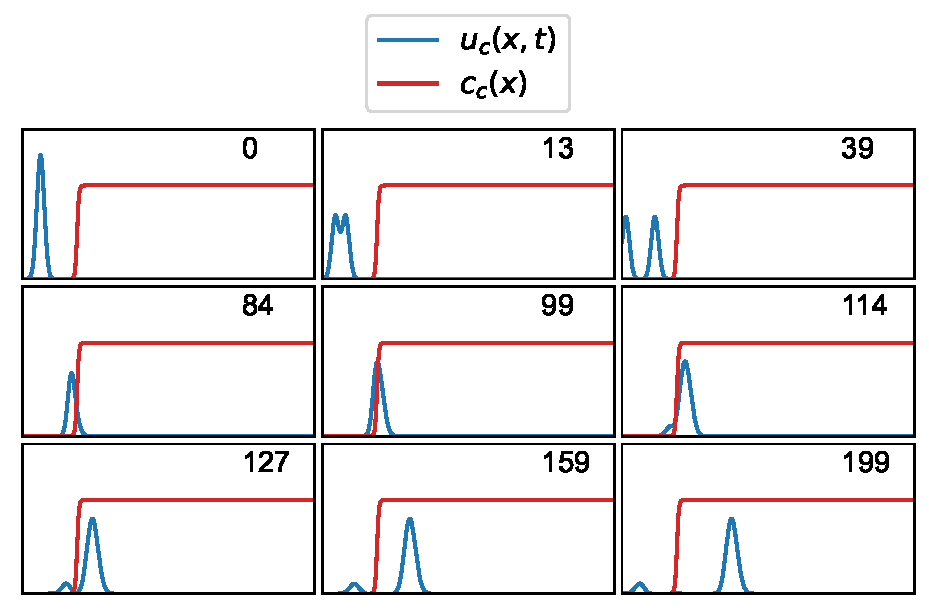
\includegraphics[clip=true,width=\columnwidth]{solucion_b.pdf}
  \caption{}
   \label{fig:solucion_b}
\end{figure}

\begin{figure}[h]
  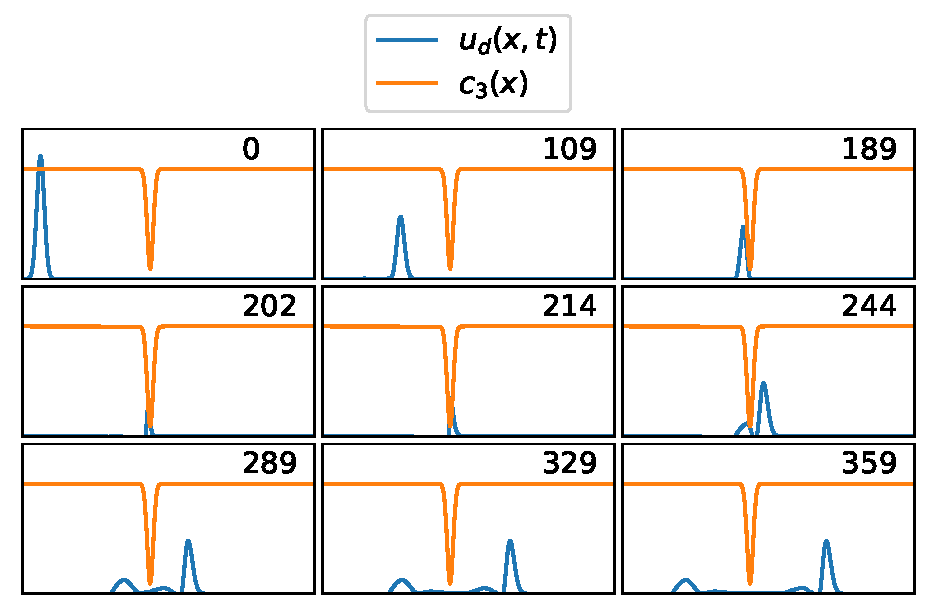
\includegraphics[clip=true,width=\columnwidth]{solucion_d.pdf}
  \caption{}
   \label{fig:solucion_d}
\end{figure}


\onecolumngrid

\begin{figure}
  \centering
  \begin{subfigure}[b]{0.45\textwidth}
      \centering
      \includegraphics[width=\textwidth]{divergencia_a.pdf}
      \caption{\label{fig:divergencia_a}}
  \end{subfigure}
  \hfill
  \begin{subfigure}[b]{0.45\textwidth}
      \centering
      \includegraphics[width=\textwidth]{divergencia_b.pdf}
      \caption{\label{fig:divergencia_b}}
  \end{subfigure}
  \hfill
  \begin{subfigure}[b]{0.45\textwidth}
      \centering
      \includegraphics[width=\textwidth]{divergencia_c.pdf}
      \caption{\label{fig:divergencia_c}}
  \end{subfigure}
  \hfill
  \begin{subfigure}[b]{0.45\textwidth}
      \centering
      \includegraphics[width=\textwidth]{divergencia_d.pdf}
      \caption{\label{fig:divergencia_d}}
  \end{subfigure}
     \caption{\textcolor{blue}{Divergencias}.}
     \label{fig:simple_error_vs_h}
\end{figure}

\twocolumngrid

% \hfill

\section{Conclusión}



\bibliography{Chehade_guia3.bib}

\end{document}





